% !TeX spellcheck = en_GB
\begin{wrapfigure}[19]{r}{0.44\textwidth}
	\vspace{-\normalbaselineskip}
	\centering
	\begin{subfigure}[b]{0.4\textwidth}
		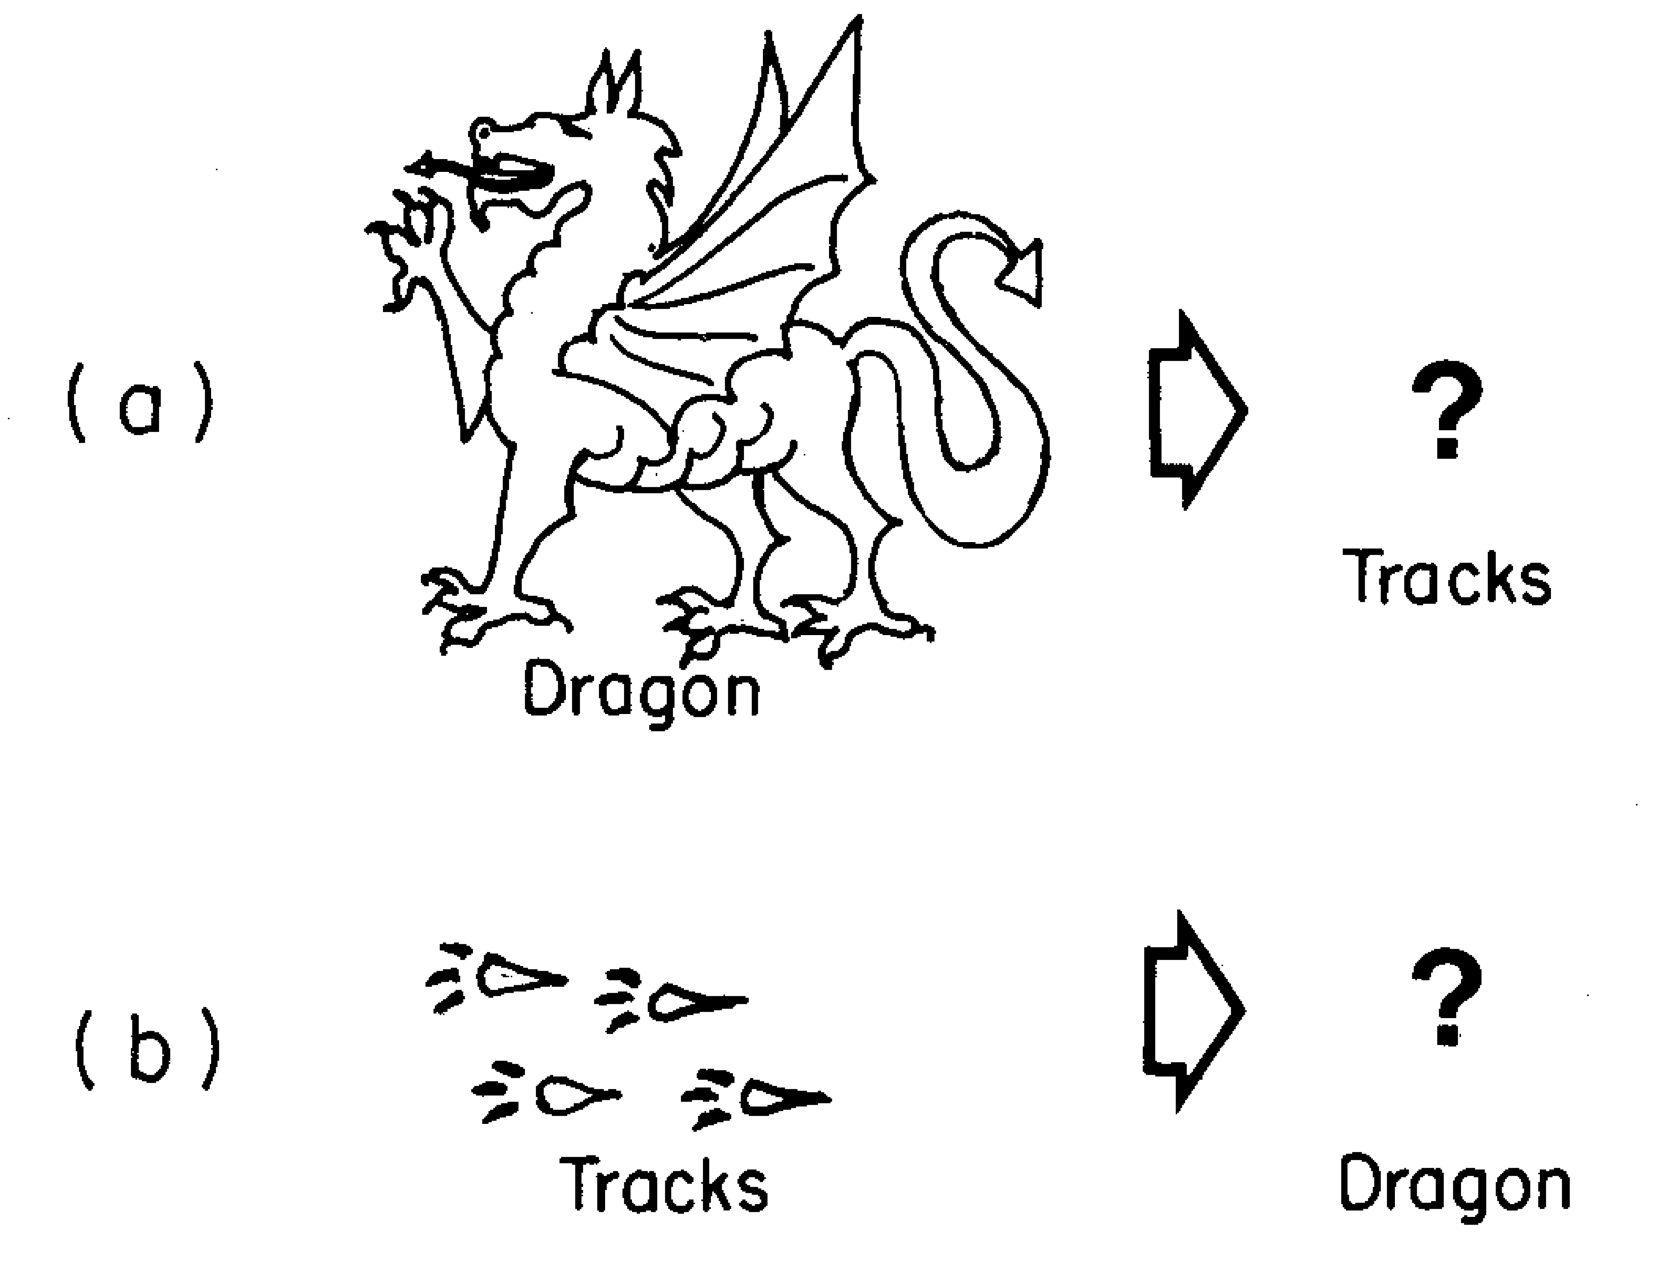
\includegraphics[trim={6cm, 8.8cm, 0cm, 0cm},clip,width=\textwidth]{./fig_instruments/Dragon_track.png}
		\caption{Forward problem.}\label{fig:dragon:forward}
	\end{subfigure}
	
	\begin{subfigure}[b]{0.4\textwidth}
		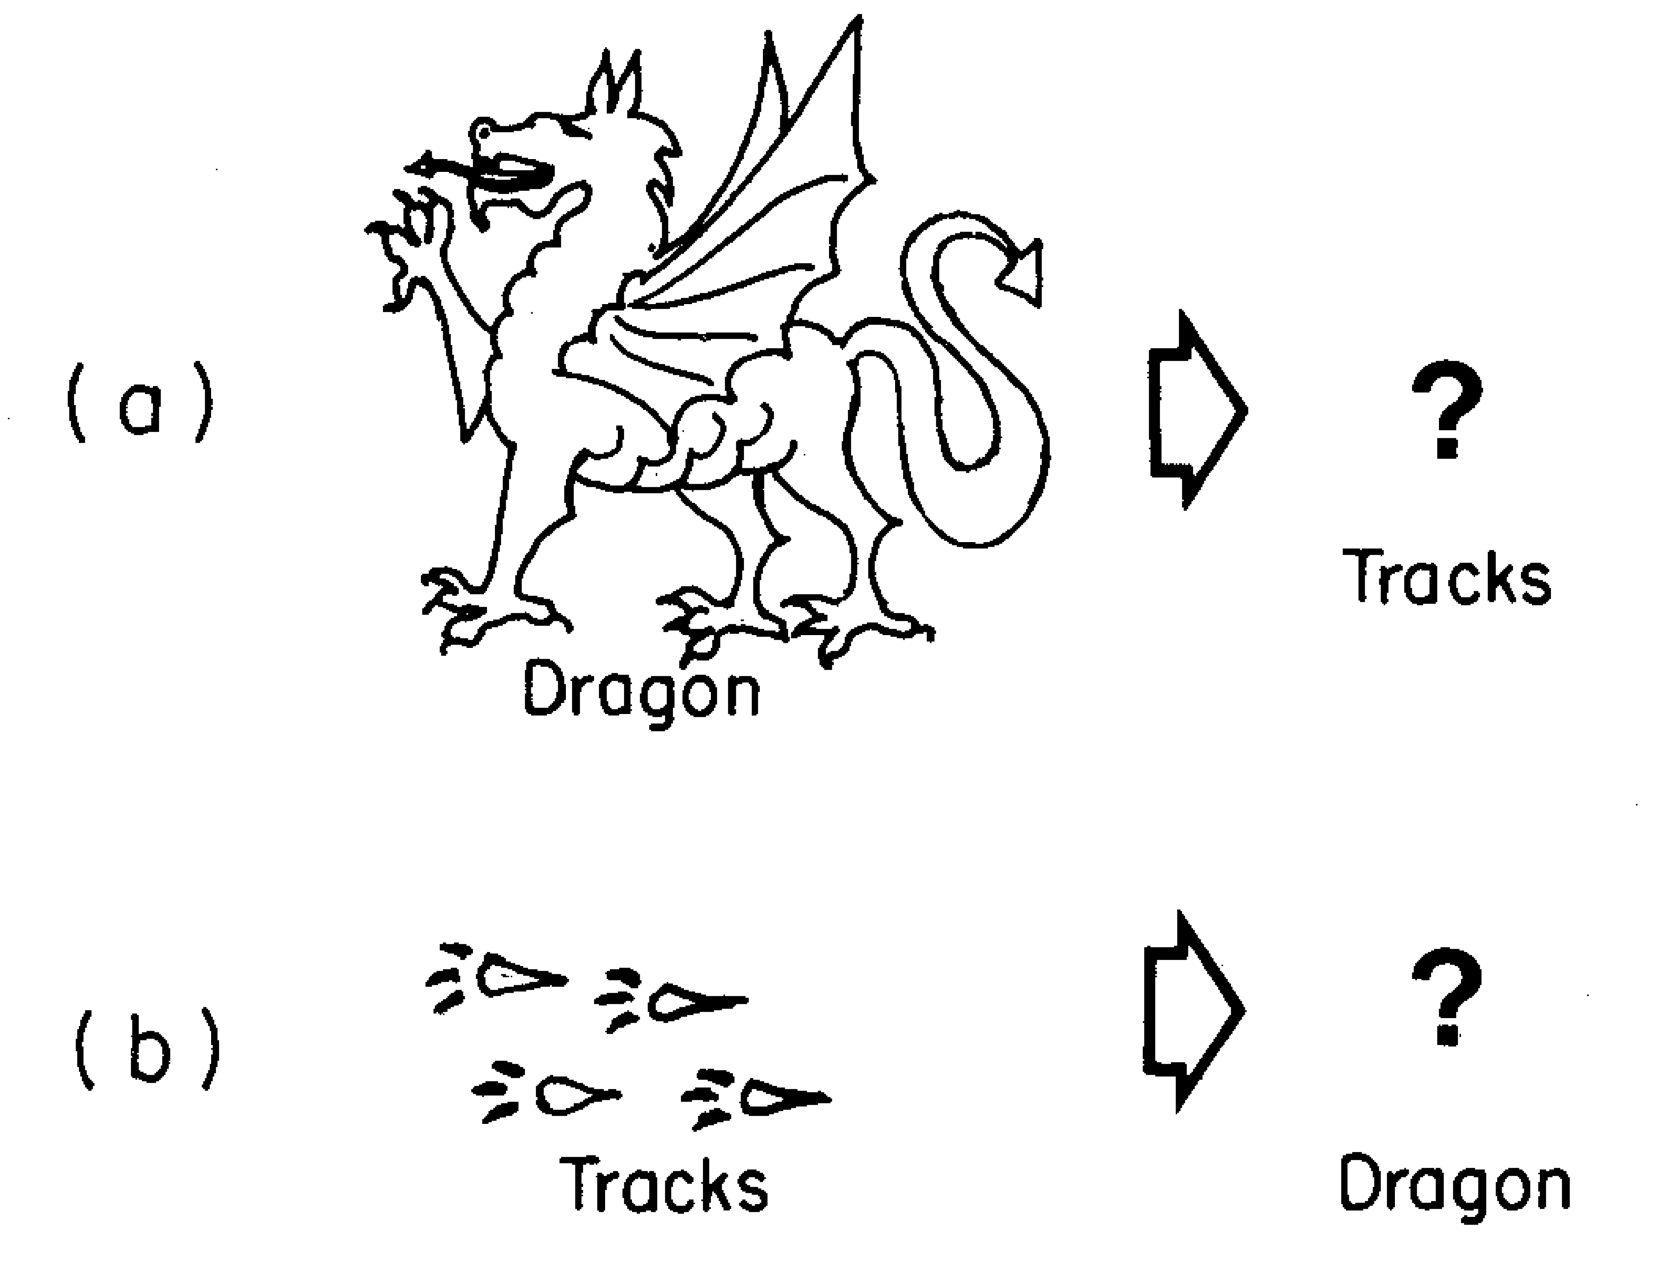
\includegraphics[trim={6cm, .8cm, 0cm, 14.8cm},clip,width=\textwidth]{./fig_instruments/Dragon_track.png}
		\caption{Inverse problem.}\label{fig:dragon:inverse}
	\end{subfigure}
	
	%	\vspace{-10pt}
	\caption{\protect\subref{fig:dragon:forward} Relationship between measurements (dragon) and the unknown parameter of interest (tracks), and \protect\subref{fig:dragon:inverse} presenting the inverse problem when the parameter of interest is known but measurements are not \citep{stephens_remote_1994}.}\label{fig:dragon}
	\vspace{-\normalbaselineskip} 
\end{wrapfigure}

% \begin{figure}[h!]
% 	\centering
%     \begin{subfigure}[b]{0.49\textwidth}
%     	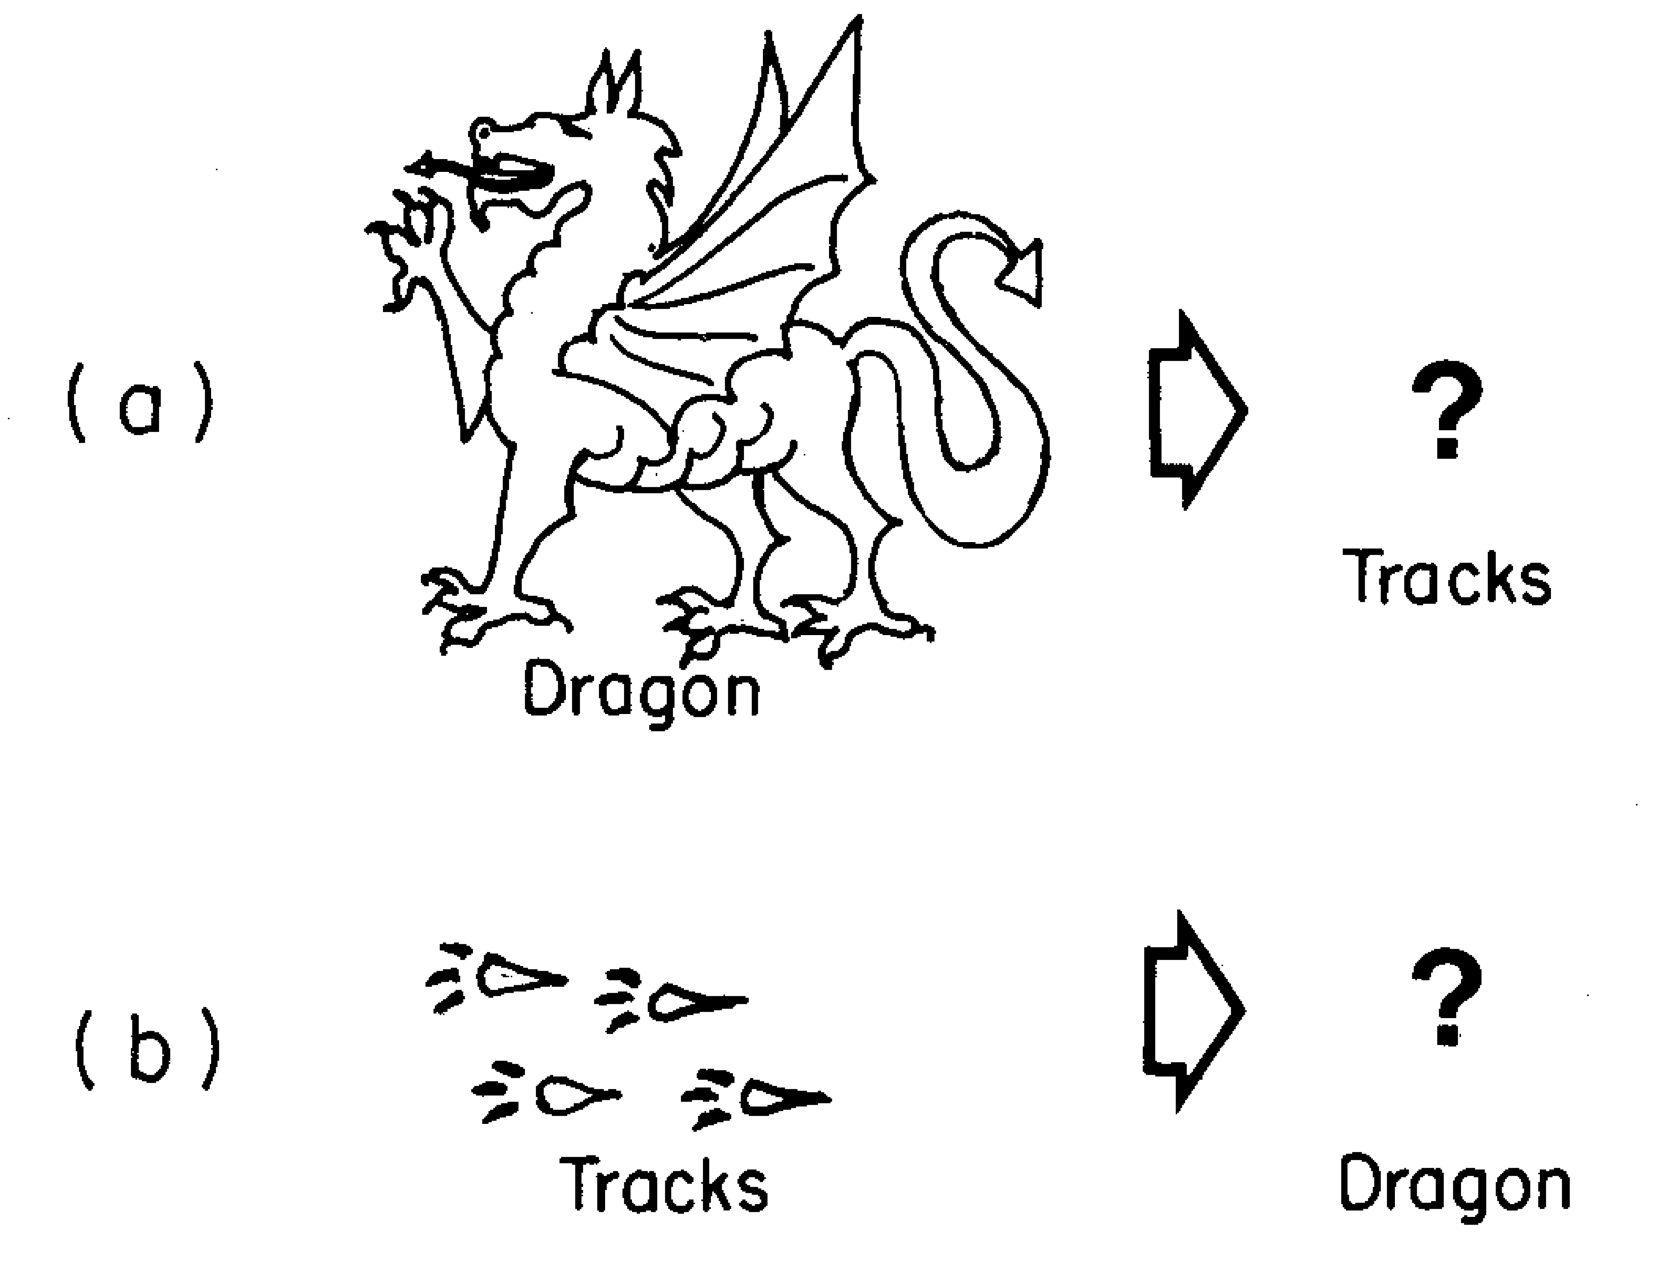
\includegraphics[trim={6cm, 8.8cm, 0cm, 0cm},clip,width=\textwidth]{./fig_instruments/Dragon_track.png}
%         \caption{Forward problem.}\label{fig:dragon:forward}
%     \end{subfigure}
%     %
%     \begin{subfigure}[b]{0.49\textwidth}
%     	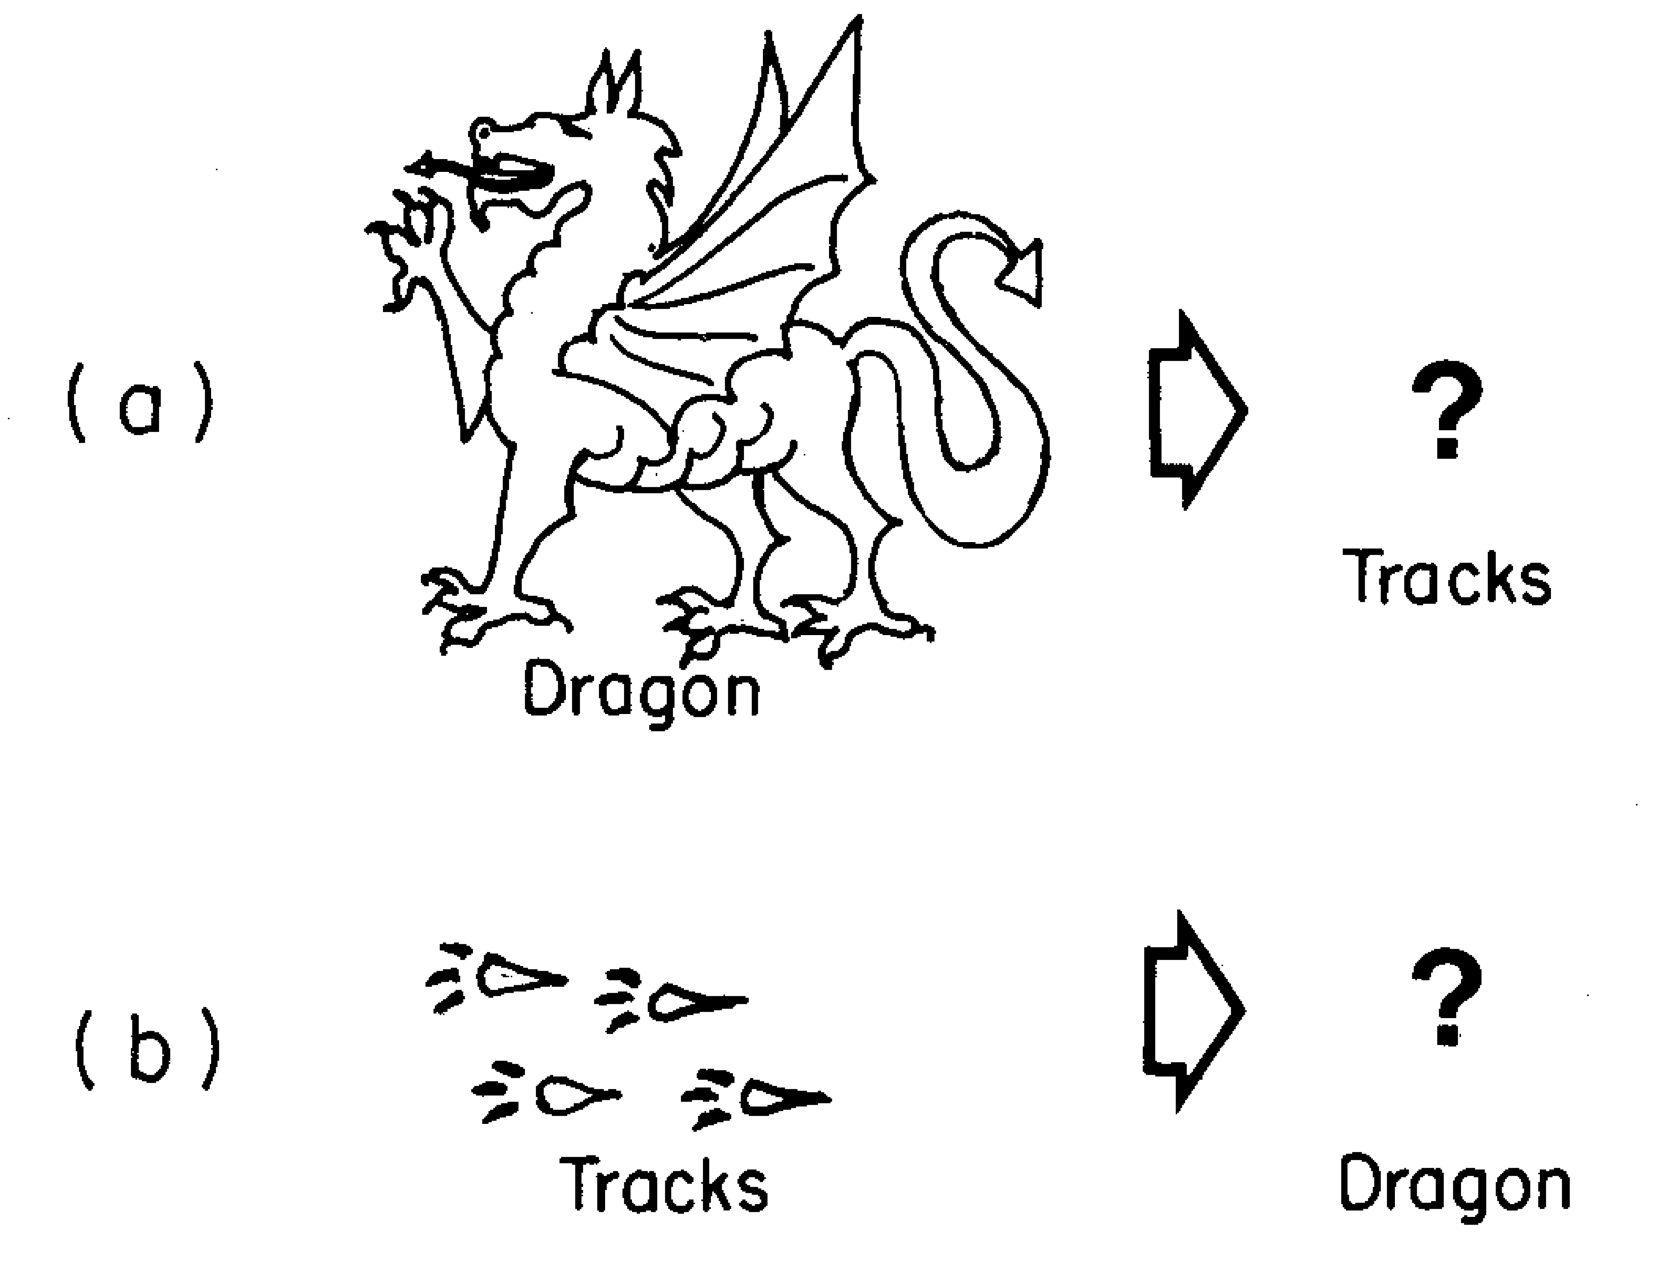
\includegraphics[trim={6cm, .8cm, 0cm, 14.8cm},clip,width=\textwidth]{./fig_instruments/Dragon_track.png}
%         \caption{Inverse problem.}\label{fig:dragon:inverse}
%     \end{subfigure}

% \end{figure}